\section{Implementacija}

\subsection{Arhitektura projekta}
Projekt Sembot sastoji se od dva glavna dijela: backend i frontend. Backend je izgrađen koristeći FastAPI, Python framework koji omogućuje brzu izradu API-ja s visokim performansama. Semantic Router koristi OpenAI-jeve embeddinge za pretvaranje upita i pitanja u vektorske reprezentacije, omogućujući semantičko pretraživanje. Podaci se pohranjuju u JSON datoteku (qa\_data.json), koja služi kao jednostavna baza podataka. Frontend je implementiran kao web aplikacija koristeći HTML, CSS i JavaScript, pružajući korisnicima jednostavno sučelje za interakciju s chatbotom.

\begin{figure}
    \centering
    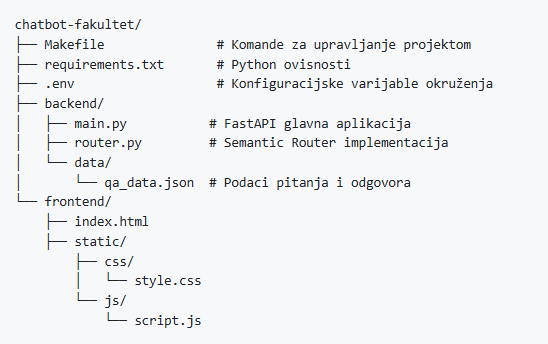
\includegraphics[width=1\linewidth]{hijerarhija.png}
    \caption{Struktura projekta}
    \label{fig:enter-label}
\end{figure}

\subsection{Prednosti arhitekture}

\begin{enumerate}
    \item Modularnost: Backend i frontend su odvojeni, što olakšava održavanje i nadogradnju.
    \item Skalabilnost: FastAPI omogućuje brzu obradu velikog broja upita.
    \item Proširivost: Novi parovi pitanje-odgovor mogu se dodati u JSON datoteku bez promjene koda.
\end{enumerate}

\begin{figure}
    \centering
    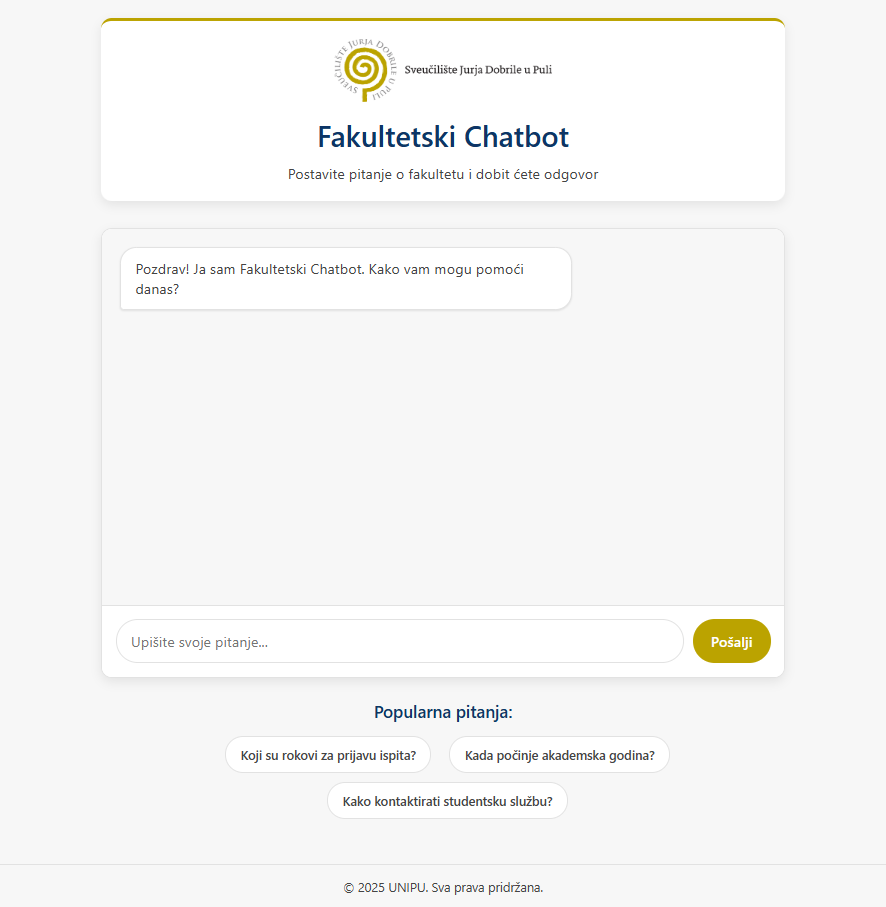
\includegraphics[width=1\linewidth]{sembot_1.png}
    \caption{Početno sučelje aplikacije}
    \label{fig:enter-label}
\end{figure}

\begin{figure}
    \centering
    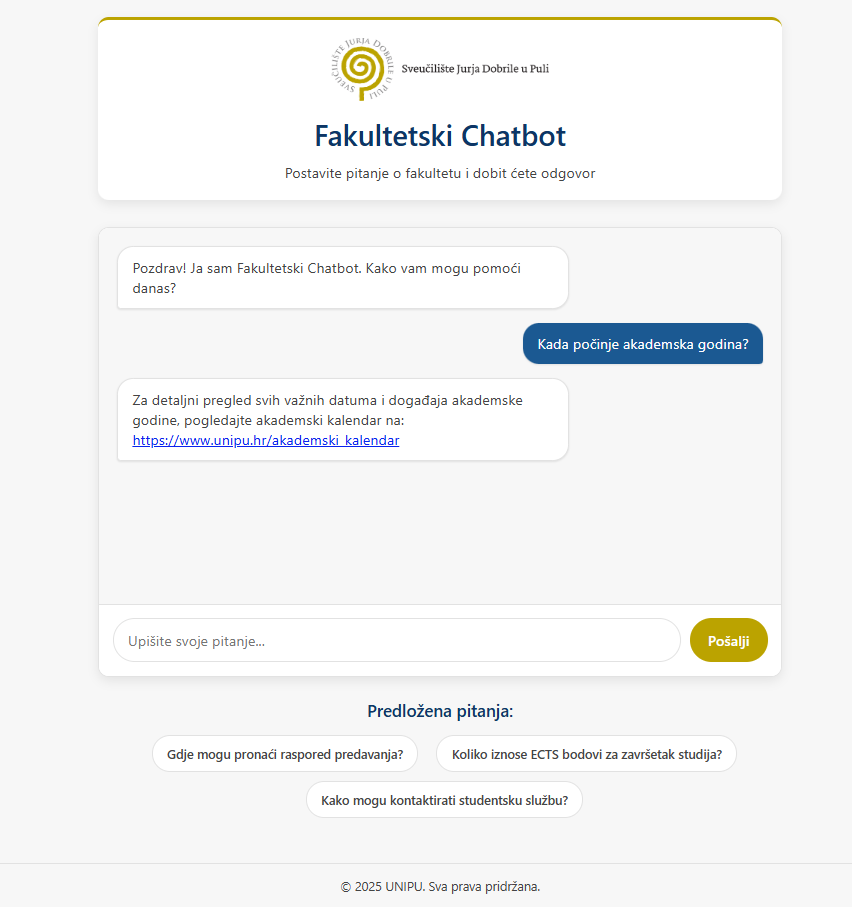
\includegraphics[width=1\linewidth]{sembot_2.png}
    \caption{Odgovor na pitanje s url linkom}
    \label{fig:enter-label}
\end{figure}

\begin{figure}
    \centering
    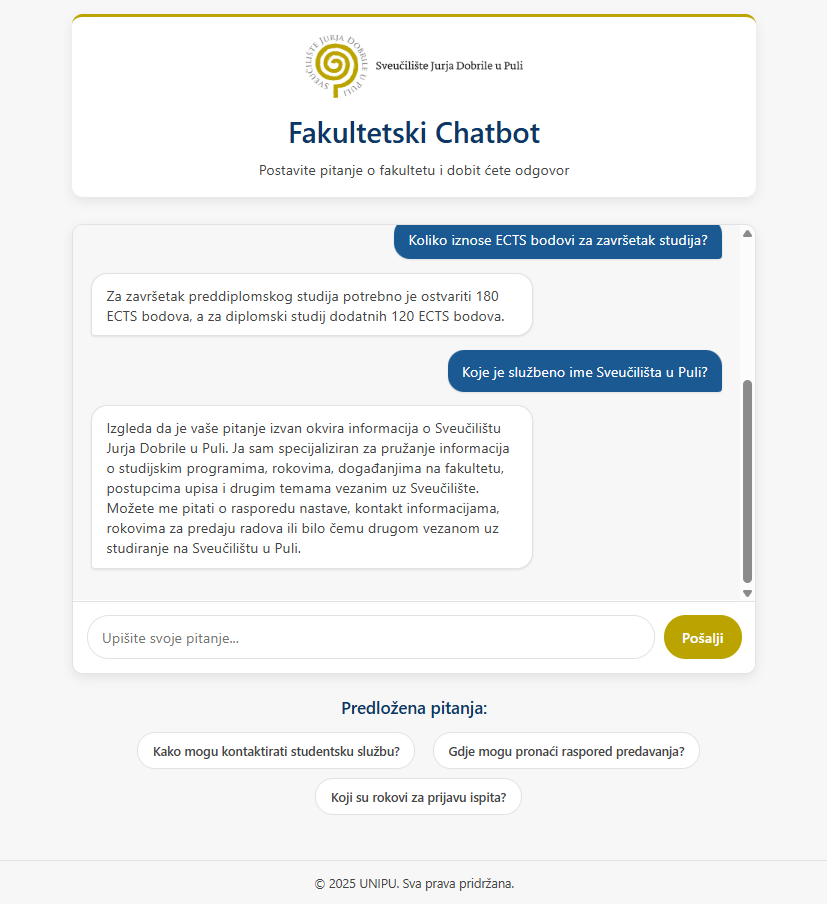
\includegraphics[width=1\linewidth]{sembot_3.png}
    \caption{Odgovor na pitanje bez url linka}
    \label{fig:enter-label}
\end{figure}

\begin{figure}
    \centering
    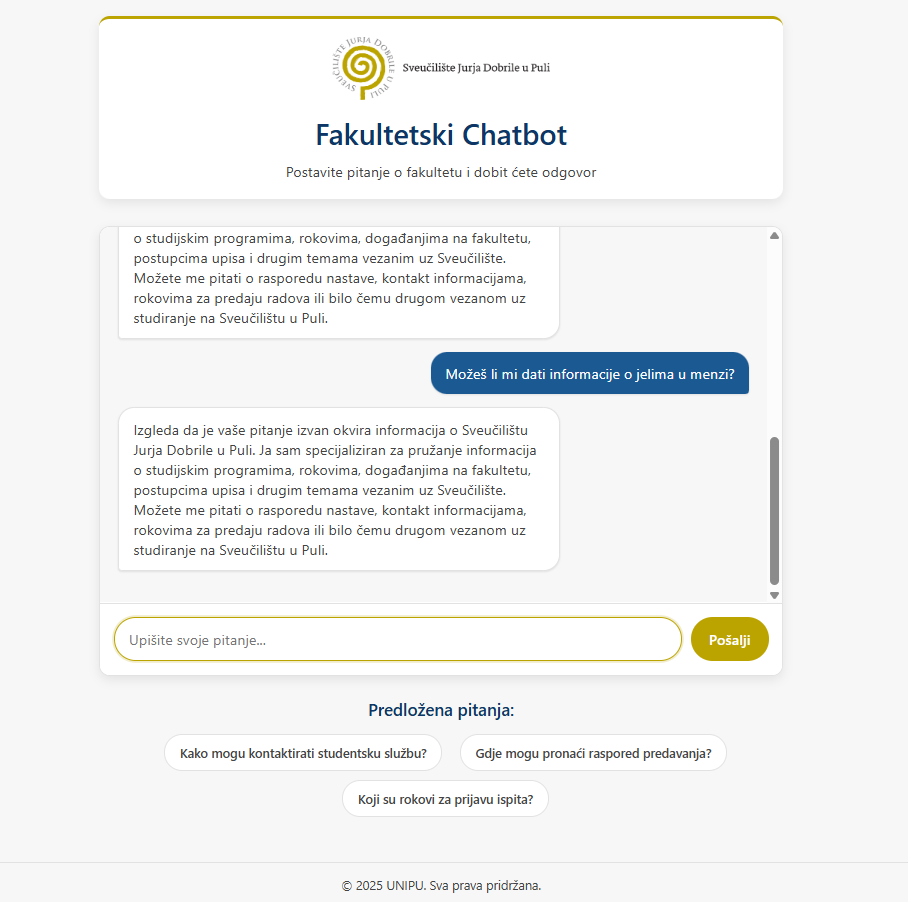
\includegraphics[width=1\linewidth]{sembot_4.png}
    \caption{Prikaz default odgovora}
    \label{fig:enter-label}
\end{figure}